%&latex
\documentclass[letterpaper,11pt]{article}
\usepackage{graphicx}
\usepackage[margin=1.0in]{geometry}
\usepackage[hyphens]{url}

\makeatletter
\setlength{\@fptop}{0pt}
\makeatother

\title{Bamsurgeon: Methods for spike-in mutations on BAM files}
\author{Adam D. Ewing (ewingad@soe.ucsc.edu)}
\begin{document}
 \date{November 7, 2013}
 \maketitle

\section{Adding SNVs to existing BAM alignments (addsnv)}
\subsection{Usage}
\begin{verbatim}
usage: addsnv.py [-h] -v VARFILENAME -f BAMFILENAME -r REFFASTA -o OUTBAMFILE
                 [-s SNVFRAC] [-m MUTFRAC] [-n NUMSNVS] [-c CNVFILE]
                 [-d COVERDIFF] [-p PROCS] [--nomut] [--det] [--force]
                 [--single]

adds SNVs to reads, outputs modified reads as .bam along with mates

optional arguments:
  -h, --help            show this help message and exit
  -v VARFILENAME, --varfile VARFILENAME
                        Target regions to try and add a SNV, as BED
  -f BAMFILENAME, --sambamfile BAMFILENAME
                        sam/bam file from which to obtain reads
  -r REFFASTA, --reference REFFASTA
                        reference genome, fasta indexed with bwa index -a
                        stdsw _and_ samtools faidx
  -o OUTBAMFILE, --outbam OUTBAMFILE
                        .bam file name for output
  -s SNVFRAC, --snvfrac SNVFRAC
                        maximum allowable linked SNP MAF (for avoiding
                        haplotypes) (default = 1)
  -m MUTFRAC, --mutfrac MUTFRAC
                        allelic fraction at which to make SNVs (default = 0.5)
  -n NUMSNVS, --numsnvs NUMSNVS
                        maximum number of mutations to try (default: entire
                        input)
  -c CNVFILE, --cnvfile CNVFILE
                        tabix-indexed list of genome-wide absolute copy number
                        values (e.g. 2 alleles = no change)
  -d COVERDIFF, --coverdiff COVERDIFF
                        allow difference in input and output coverage
                        (default=0.9)
  -p PROCS, --procs PROCS
                        split into multiple processes (default=1)
  --nomut               dry run
  --det                 deterministic base changes: make transitions only
  --force               force mutation to happen regardless of nearby SNP or
                        low coverage
  --single              input BAM is simgle-ended (default is paired-end)

\end{verbatim}

\subsection{Description}
    Single nucleotide changes are introduced to an existing BAM alignment using \texttt {addsnv.py} as described in Figure 4. Input consists of a list of locations where SNVs will be made, a target BAM alignment, and a reference genome indexed using bwa (preferably the same genome used to align the reads in the BAM file). Additionally there are a number of optional arguments, including the option to make deterministic mutations (default is random, deterministic always makes transitions), an option to skip locations if a SNP above a specified MAF is located nearby (avoid interfering with haplotypes), and the MAF of the spike-in SNVs (default 0.5/heterozygous). Output consists of a BAM file containing the spike-in mutations and a directory of log files describing which bases were changed in which reads (one log per mutation). Currently, the directory containing output logs can be transformed into VCF format using the script \texttt {makevcf.py} in the \texttt {etc/} subdirectory. The spike-in process may be multithreaded through the sue of the \texttt {-p / --procs} option.

\begin{figure}[!h]
\centering
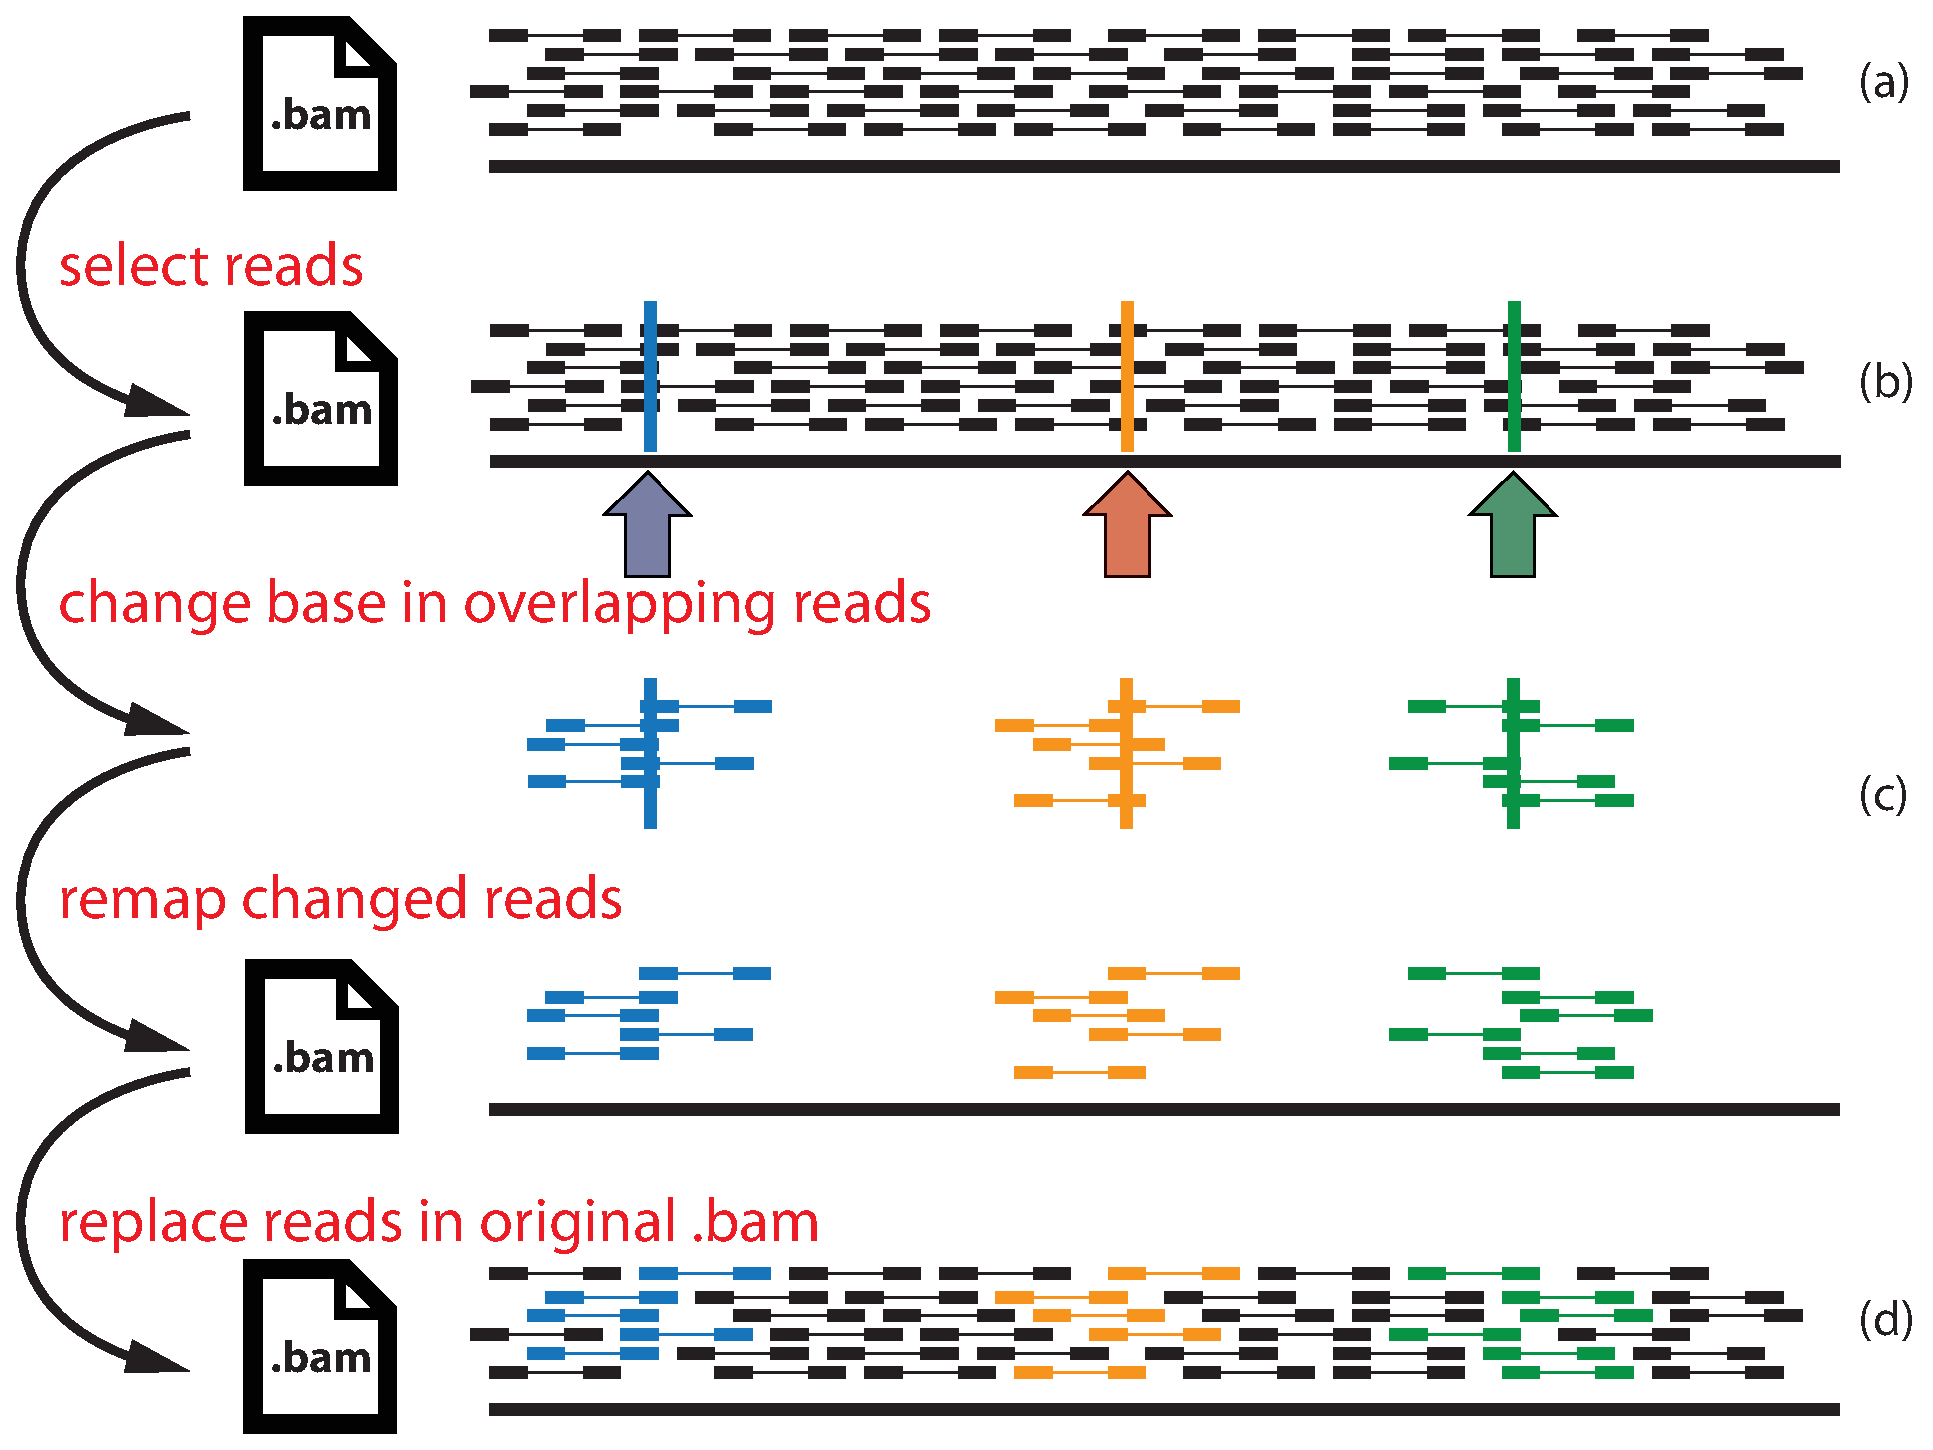
\includegraphics[width=5.5in]{bamsurgeon_snv.eps}
\caption{Method for adding SNVs to existing BAM alignments. Starting with the original BAM alignment (a) and a list of positions (b), reads overlapping the chosen positions are selected the target base change is made (c). Altered reads are re-mapped the the reference genome using bwa, and the modified, realigned reads replace the unmodified versions in the original BAM (d).}
\end{figure}

\section{Adding indels and SVs to existing BAM alignments (addsv.py)}

\subsection{Usage}
\begin{verbatim}
usage: addsv.py [-h] -v VARFILENAME -f BAMFILENAME -r REFFASTA -o OUTBAMFILE
                [-l MAXLIBSIZE] [-k KMERSIZE] [-s SVFRAC]
                [--maxctglen MAXCTGLEN] [-n MAXMUTS] [-c CNVFILE] [-p PROCS]
                [--nomut] [--noremap] [--noref] [--recycle]

adds SNVs to reads, outputs modified reads as .bam along with mates

optional arguments:
  -h, --help            show this help message and exit
  -v VARFILENAME, --varfile VARFILENAME
                        whitespace-delimited target regions to try and add a
                        SNV: chrom,start,stop,action,seqfile if
                        insertion,TSDlength if insertion
  -f BAMFILENAME, --sambamfile BAMFILENAME
                        sam/bam file from which to obtain reads
  -r REFFASTA, --reference REFFASTA
                        reference genome, fasta indexed with bwa index -a
                        stdsw _and_ samtools faidx
  -o OUTBAMFILE, --outbam OUTBAMFILE
                        .bam file name for output
  -l MAXLIBSIZE, --maxlibsize MAXLIBSIZE
                        maximum fragment length of seq. library
  -k KMERSIZE, --kmer KMERSIZE
                        kmer size for assembly (default = 31)
  -s SVFRAC, --svfrac SVFRAC
                        allele fraction of variant (default = 1.0)
  --maxctglen MAXCTGLEN
                        maximum contig length for assembly - can increase if
                        velvet is compiled with LONGSEQUENCES
  -n MAXMUTS            maximum number of mutations to make
  -c CNVFILE, --cnvfile CNVFILE
                        tabix-indexed list of genome-wide absolute copy number
                        values (e.g. 2 alleles = no change)
  -p PROCS, --procs PROCS
                        split into multiple processes (default=1)
  --nomut               dry run
  --noremap             dry run
  --noref               do not perform reference based assembly
  --recycle

\end{verbatim}

\subsection{Description}
    Small insertions and deletions (indels), and larger structural variants (insertions, deletions, duplications, inversions, and compound variants) are added to existing BAM alignments using \texttt{addsv.py} as described in Figure 5. Input consists of a list of regions where SVs will be made along with a specification of each variant, a target BAM alignment, and a reference genome indexed using bwa.
    The input mutation list consists of four columns: chromosome, start of region, end of region, and a controlled-vocabulary description of the mutation. A mutation will not be made if the largest contig obtained from local assembly of the specified region is less than 3 times the maximum expected library size (specified by \texttt{-l/--maxlibsize}). The mutation description starts with either \texttt{INS, DEL, DUP}, or \texttt{INV} for insertion, deletion, duplication, and inversion, respectively and is followed by mutation-specific options.

    For insertions, \texttt{INS} should be followed by either a FASTA file containing the sequence to be inserted, or by the nucleotide sequence itself. For example, \texttt{INS ATG} would insert the sequence \texttt{``ATG''} in the middle of the largest contig obtained from the specified region, while \texttt{INS LINE1.fa} would insert the sequence in the FASTA-formatted file \texttt{LINE1.fa} into the largest contig. For deletions, \texttt{DEL} should be followed by the fraction of the largest contig to be deleted, where 1.0 indicates a deletion of the largest assembled region minus one library length on each end. e.g. {DEL 0.5}. Inversions (\texttt{INV}) have no further options - the region inside the largest contig will be inverted. Duplications (\texttt{DUP}) have one optional parameter, an integer specifying the number of times the sequence of the largest contig should be duplicated, e.g. \texttt{DUP 2} specifies the region is duplicated twice.

    Compound variants are also possible by chaining a number of mutations together in a comma-delimited list, e.g. \texttt{DUP 1, DEL 0.5, INS AAATCC, INV} would duplicate the region inside the largest contig once, delete half the width of the region, insert the sequence \texttt{AAATCC}, and invert the region.
    
    Where mutations add sequence (e.g. duplications), new reads are created that will be added to the original BAM, and where mutations remove sequence (e.g. deletions) those reads are maked as excluded (excluded read names are recorded in the file specified by \texttt{-x/--excluded}). Excluded reads are not carried over from the original BAM to the mutated BAM, creating the copy number effect associated with deletion.
    
     Output consists of a BAM file containing the spike-in mutations and a directory of log files describing which bases were changed in which reads (one log per mutation) and the local assemblies for each region where a mutation was made. Currently, the directory containing output logs for SV spike-ins can be transformed into VCF format using the script \texttt {makevcf\_sv.py} in the \texttt {etc/} subdirectory. The spike-in process may be multithreaded through the sue of the \texttt {-p / --procs} option.

\begin{figure}[!h]
\centering
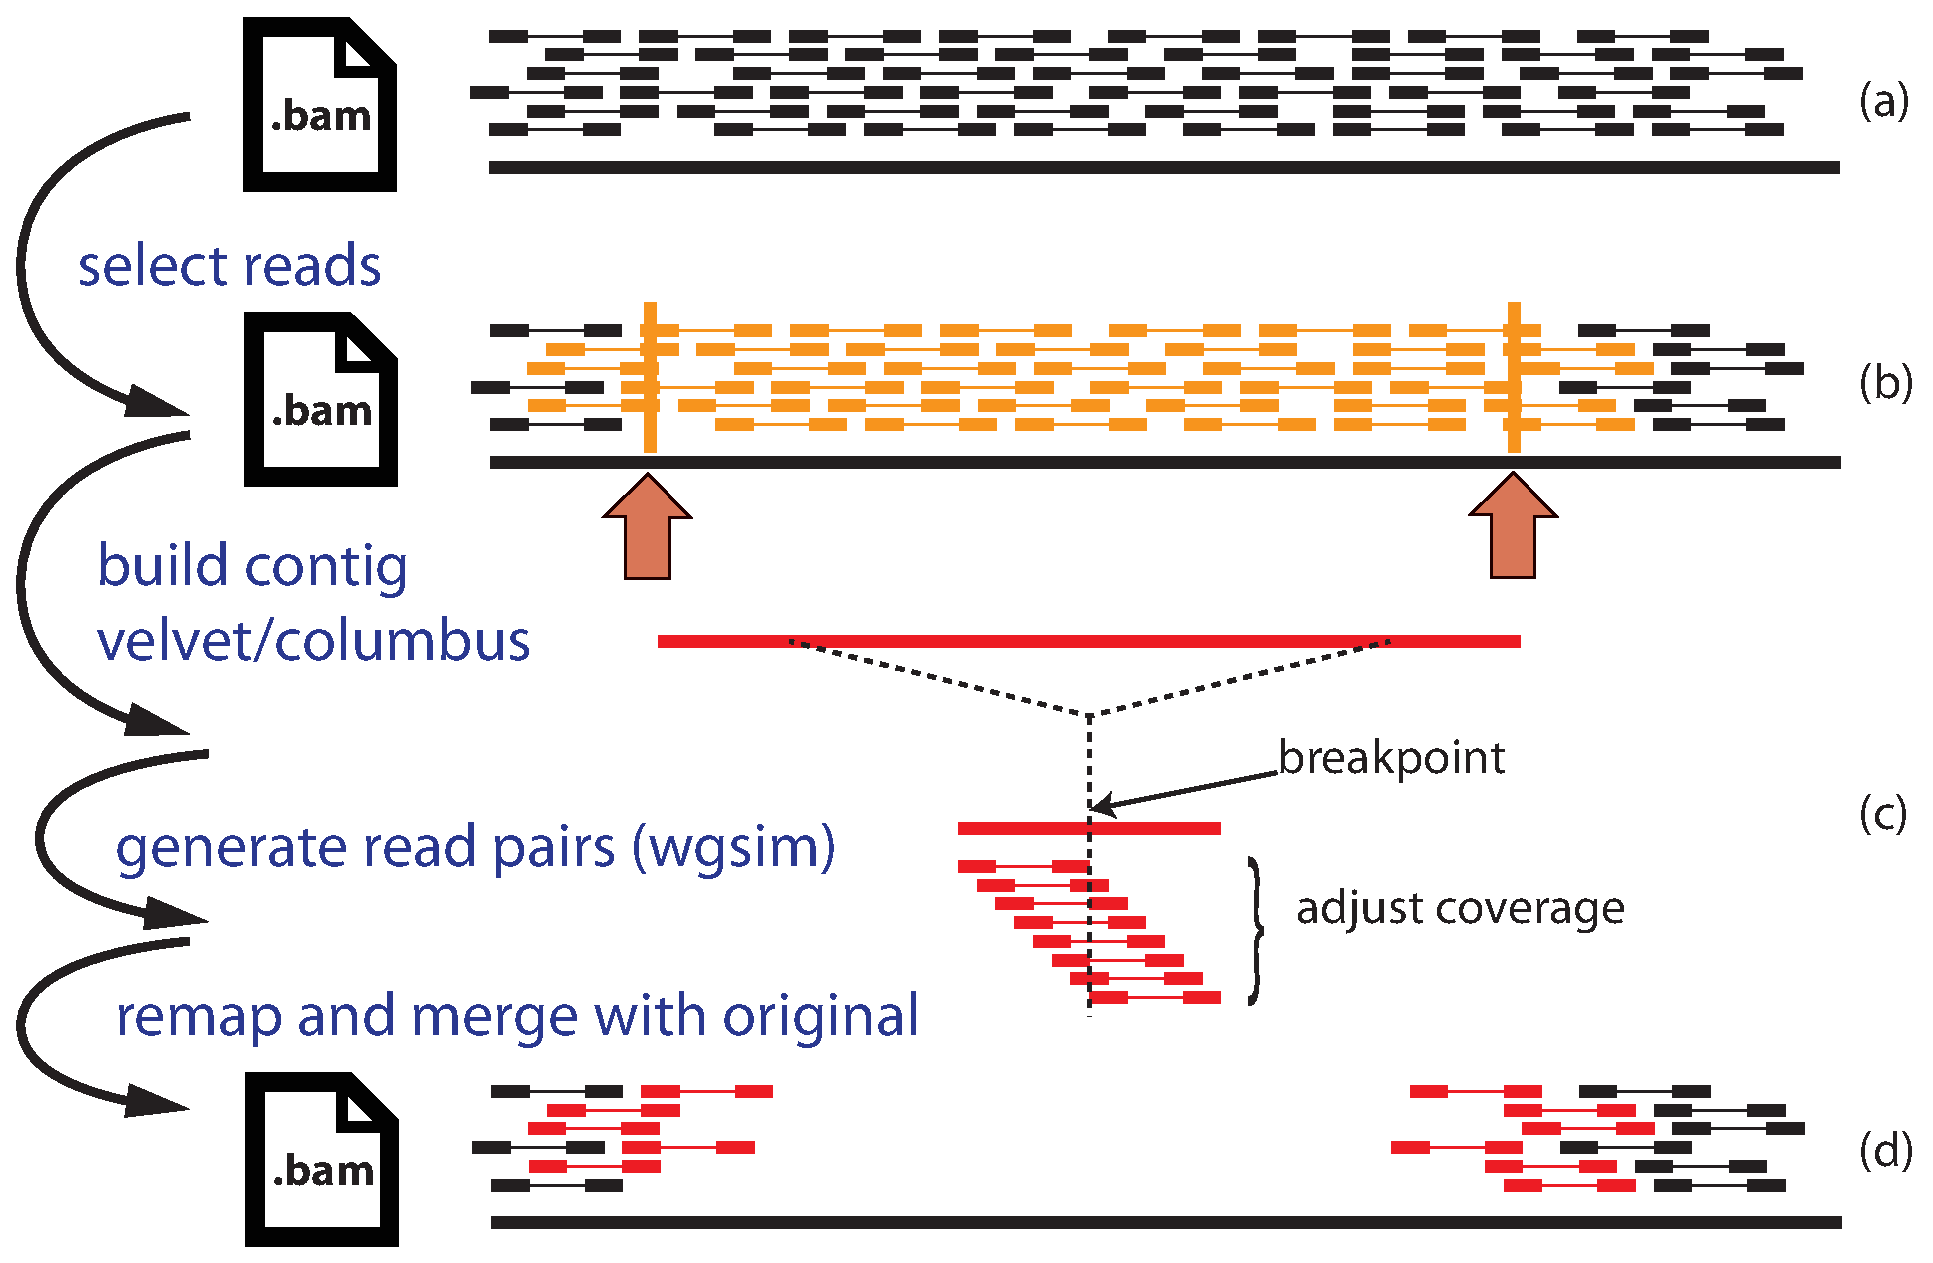
\includegraphics[width=5.5in]{bamsurgeon_sv_del.eps}
\caption{Method for adding multi-nucleotide variants (indels and SVs) to existing BAMs: deletion example. Starting with the original BAM alignment (a) regions, e.g. (b), are assembled using Velvet/Columbus (\texttt{http://www.ebi.ac.uk/~zerbino/velvet/}) and the desired mutation(s) are created in the largest contig. Read coverage is simulated over the contig using wgsim (\texttt{https://github.com/lh3/wgsim}, also included with samtools) with parameters \texttt{-e 0 -r 0 -R 0} to suppress additional mutations, other parameters are set based on the input BAM and desired coverage. Simulated coverage is scaled based on whether the mutation is adds sequence (duplication) or removes sequence (deletions), and replaced into the original BAM while excluded reads are removed from the original BAM (d).}
\end{figure}

\end{document}
